\documentclass{article} % Tamaño de fuente 12pt

% \usepackage[utf8]{inputenc} % Codificación de caracteres
\usepackage[spanish]{babel} % Idioma español
\usepackage{graphicx} % Para incluir imágenes
\usepackage{hyperref} % Para enlaces (opcional)
\usepackage{comment} % Para comentarios
\usepackage{enumitem} % Para negrita en listas
\usepackage[letterpaper, left=1in, right=1in, top=1in, bottom=1in, headheight=1.5in]{geometry}
\usepackage{fancyhdr} % Para incluir imágenes en el encabezado

% Información básica
\title{Documentación del Proyecto de Horarios}
\author{Janer Alberto Vega Jácome}
\date{\today}

\begin{comment}    
%Definiendo estilo del encabezado
\fancypagestyle{mystyle}{
    \fancyhf{} % Limpia el encabezado y pie de página
    \renewcommand{\headrulewidth}{0pt} % Elimina la línea horizontal del encabezado
    \fancyhead[L]{
\includegraphics[width=2cm]{Imágenes/logoEscuela.png}}
    \fancyhead[C]{ % Títulos del encabezado
        \begin{minipage}{0.7\textwidth} % Ajusta el ancho del minipage para los títulos
            \centering
            \raisebox{0in}{
                {\large Escuela de Ingeniería de Sistemas e Informática}
            }
            \raisebox{0cm}{
                {\small Universidad Industrial de Santander}
            }
        \end{minipage}
    }
    \fancyhead[R]{
\includegraphics[width=3.5cm]{Imágenes/logoUIS.png}}

    \fancyfoot[C]{\thepage} % Número de página centrado
    
}

% Aplicando el estilo del encabezado y pie de página
\pagestyle{mystyle}
\end{comment}

\begin{document}

\maketitle % Crea la portada con título, autor y fecha

\newpage
\section{Requerimientos}
\subsection{Idea general}
\noindent
El proyecto de horarios tiene como objetivo desarrollar una aplicación web que permita a los usuarios crear, gestionar y visualizar horarios de manera eficiente. Utilizando Spring Boot para el backend y Angular para el frontend, esta aplicación ofrecerá una interfaz intuitiva y funcionalidades avanzadas para la gestión de horarios.
\begin{comment}
\subsection{Equipo de Desarrollo}
\begin{table}[h!]
\centering
\begin{tabular}{|l|l|}
\hline
\textbf{Nombre} & \textbf{Rol} \\ \hline
Juan Alarcon & Desarrollador Front-End \\ \hline
Diego Medina & Desarrollador Back-End \\ \hline
Janer Vega & Documentación \\ \hline
\end{tabular}
\end{table}
\end{comment}

\subsection{Objetivos}
    \subsubsection{Objetivo general}
    \noindent
    Desarrollar un sistema de gestión de horarios académicos para la Escuela de Ingeniería de Sistemas e Informática de la UIS que automatice y optimice la planificación, asignación y visualización de horarios y considerando las restricciones de recursos (aulas, profesores) con el fin de mejorar la eficiencia y transparencia del proceso académico.
    \subsubsection{Objetivos específicos}
    \begin{enumerate}[font=\bfseries] % Aplica negrita a los números
        \item \textbf{Interfaz de Usuario:} Diseñar una interfaz gráfica de usuario (GUI) intuitiva y fácil de usar que permita a los usuarios (administradores, profesores y estudiantes) interactuar con el sistema de manera eficiente, proporcionando módulos específicos para la gestión de usuarios, registro académico y diseño de horarios.
        \item \textbf{Gestión de Usuarios:} Implementar un módulo de gestión de usuarios que permita el registro, autenticación, autorización y administración de perfiles de usuarios (administradores, profesores, estudiantes, técnicos, auxiliares, secretarias), asignando roles y permisos adecuados para cada tipo de usuario.
        \item \textbf{Registro Académico:} Desarrollar un sistema de registro académico que permita la gestión de información relevante para la generación de horarios, incluyendo:
        \begin{itemize}
            \item Asignaturas: Nombre, código, créditos, tipo (teórica, práctica, laboratorio).
            \item Profesores: Nombre, identificación, disponibilidad horaria, preferencias de asignaturas.
            \item Aulas: Nombre, capacidad, tipo (aula de clase, laboratorio), disponibilidad horaria.
            \item Grupos: Identificación, número de estudiantes, asignaturas asociadas.
        \end{itemize}
        \item \textbf{Algoritmo de Diseño de Horarios:} Diseñar e implementar un algoritmo eficiente y flexible para la generación automática de horarios académicos que considere:
        \begin{itemize}
            \item Restricciones de recursos: Disponibilidad de aulas y profesores en diferentes horarios.
            \item Restricciones académicas: Carga horaria de profesores, número máximo de estudiantes por grupo.
            \item Métricas de optimización: Minimizar conflictos de horarios, maximizar la utilización de recursos, equilibrar la carga horaria de profesores.
        \end{itemize}
        \item \textbf{Generación de Reportes:} Desarrollar un módulo de generación de reportes que permita visualizar y exportar horarios en diferentes formatos (PDF, Excel) para:
        \begin{itemize}
            \item Profesores: Horario individual por profesor.
            \item Aulas: Horario de ocupación de cada aula.
            \item Asignaturas: Horario de cada asignatura, incluyendo grupos y profesores.
            \item Horario General: Horario completo de la Escuela, mostrando todas las asignaturas, grupos, profesores y aulas.
        \end{itemize}
    \end{enumerate}
    
\subsection{Usuarios}
\noindent
El sistema de gestión de horarios está diseñado para ser utilizado por los siguientes grupos de usuarios dentro de la Escuela de Ingeniería de Sistemas de la UIS:
    \subsubsection{Estudiantes}
    \noindent
    Los estudiantes son los principales beneficiarios del sistema. Utilizarán la aplicación para consultar sus horarios de clases, incluyendo aulas, profesores y horarios de cada materia. 
    
    \subsubsection{Profesores}
    \noindent
    Los profesores también son usuarios clave del sistema. Utilizarán la aplicación para:
    \begin{itemize}
        \item Consultar sus horarios de clases, incluyendo aulas y grupos asignados.
        \item Reportar cambios o ajustes en sus horarios.
        \item Visualizar la disponibilidad de aulas para programar actividades adicionales.
    \end{itemize}
    
    \subsubsection{Personal administrativo}
    \noindent
    El personal administrativo de la Escuela utilizará el sistema para:
    \begin{itemize}
        \item Crear y gestionar los horarios académicos, asignando cursos, profesores y aulas.
        \item Realizar cambios y ajustes en los horarios según sea necesario.
        \item Generar reportes y estadísticas sobre la utilización de aulas y recursos.
        \item Gestionar los permisos de acceso de los usuarios al sistema.    
    \end{itemize}

\subsection{Requisitos generales}
    \subsubsection{Funcionalidad}
    \noindent
    El sistema debe permitir la creación, visualización, modificación y gestión de horarios académicos para la Escuela de Ingeniería de Sistemas e Informática de la UIS.
    \subsubsection{Usabilidad}
    \noindent
    La interfaz de usuario debe ser intuitiva, fácil de usar y accesible para todos los usuarios (administradores, profesores y estudiantes).
    \subsubsection{Rendimiento}
    \noindent
    El sistema debe ser capaz de generar horarios de manera eficiente, incluso para un gran número de asignaturas, profesores y estudiantes.
    \subsubsection{Seguridad}
    \noindent
    El sistema debe proteger la información sensible de los usuarios y garantizar que solo los usuarios autorizados puedan acceder y modificar los datos.
    \subsubsection{Escalabilidad}
    \noindent
    El sistema debe ser diseñado para adaptarse al crecimiento futuro de la Escuela, permitiendo la adición de nuevas asignaturas, profesores y estudiantes.
    \subsubsection{Compatibilidad}
    \noindent
    El sistema debe ser compatible con los navegadores web modernos (Chrome, Firefox, Safari, Edge) y funcionar en diferentes dispositivos (computadoras, tabletas, teléfonos móviles).

\subsection{Requisitos funcionales}
    \subsubsection{Gestión de usuarios}
    \begin{itemize}
        \item El sistema debe permitir el registro de nuevos usuarios (administradores, profesores, estudiantes).
        \item El sistema debe permitir la autenticación de usuarios mediante nombre de usuario y contraseña.
        \item El sistema debe asignar roles y permisos a los usuarios según su tipo (administrador, profesor, estudiante).
        \item El sistema debe permitir la modificación y eliminación de perfiles de usuario.
    \end{itemize}
    
    \subsubsection{Registro académico}
    \begin{itemize}
        \item El sistema debe permitir el registro de asignaturas, incluyendo nombre, código, créditos, prerrequisitos y tipo.
        \item El sistema debe permitir el registro de profesores, incluyendo nombre, identificación, disponibilidad horaria y preferencias de asignaturas.
        \item El sistema debe permitir el registro de aulas, incluyendo nombre, capacidad, tipo y disponibilidad horaria.
        \item El sistema debe permitir el registro de grupos, incluyendo identificación, número de estudiantes y asignaturas asociadas.
    \end{itemize}
    
    \subsubsection{Diseño de horarios}
    \begin{itemize}
        \item El sistema debe generar automáticamente horarios académicos que cumplan con las restricciones de recursos y académicas.
        \item El sistema debe permitir la modificación manual de los horarios generados.
        \item El sistema debe detectar y notificar conflictos de horarios (choques entre bloques de horas, solapamiento de horarios).
        \item El sistema debe permitir la optimización de los horarios según diferentes criterios (minimizar conflictos, maximizar la utilización de recursos, equilibrar la carga horaria de profesores).
    \end{itemize}
    
    \subsubsection{Visualización de horarios}
    \begin{itemize}
        \item El sistema debe permitir la visualización de horarios individuales por profesor.
        \item El sistema debe permitir la visualización de horarios de ocupación de aulas.
        \item El sistema debe permitir la visualización de horarios por asignatura, incluyendo grupos y profesores.
        \item El sistema debe permitir la visualización de un horario general de la Escuela.
    \end{itemize}
    
    \subsubsection{Generación de reportes}
    \begin{itemize}
        \item El sistema debe permitir la exportación de horarios en formato PDF.
        \item El sistema debe permitir la exportación de horarios en formato Excel.
    \end{itemize}

\subsection{Información de autoría}
\begin{itemize}
    \item Este proyecto es desarrollado por estudiantes de la Escuela de Ingeniería de Sistemas e Informática de la Universidad Industrial de Santander (UIS), como parte de una auxiliatura académica.
    \item Los derechos de autor del código fuente y la documentación del proyecto pertenecen a la Escuela de Ingeniería de Sistemas e Informática de la Universidad Industrial de Santander (UIS).
    % \item El proyecto se distribuye bajo una licencia de código abierto \textit{(debemos escoger una)}.
\end{itemize}

\subsection{Alcances y limitaciones}
    \subsubsection{Alcances}
    \begin{itemize}
        \item El sistema se enfocará en la gestión de horarios académicos para la Escuela de Ingeniería de Sistemas e Informática de la UIS.
        \item El sistema permitirá la generación automática de horarios, considerando restricciones y preferencias.
        \item El sistema ofrecerá diferentes vistas de horarios y la posibilidad de exportarlos en varios formatos.
    \end{itemize}
    
    \subsubsection{Limitaciones}
    \begin{itemize}
        \item El sistema no gestionará otros aspectos de la vida académica, como calificaciones, asistencia o inscripciones.
        \item El sistema no se integrará inicialmente con otros sistemas de la universidad.
        \item El algoritmo de diseño de horarios puede no encontrar soluciones óptimas en todos los casos, especialmente si las restricciones son muy complejas o contradictorias.
    \end{itemize}

\subsection{Herramientas de desarrollo}
\begin{enumerate}[font=\bfseries]
    \item \textbf{IntelliJ IDEA Ultimate}
    \begin{itemize}
        \item \textbf{Tipo:} Entorno de desarrollo integrado (IDE)
        \item \textbf{Justificación:} Para desarrollar el backend de la aplicación en Spring Boot, aprovechando sus herramientas de desarrollo Java y su integración con frameworks de Spring.
    \end{itemize}
    
    \item \textbf{Visual Studio Code (VS Code)}
    \begin{itemize}
        \item \textbf{Tipo:} Editor de código fuente
        \item \textbf{Justificación:} Para desarrollar el frontend de la aplicación en Angular, utilizando sus extensiones para Angular y TypeScript, así como sus herramientas de depuración y pruebas.
    \end{itemize}
    
    \item \textbf{MySQL Workbench}
    \begin{itemize}
        \item \textbf{Tipo:} Herramienta de administración de bases de datos
        \item \textbf{Justificación:} Para diseñar y administrar la base de datos MySQL donde se almacenarán los datos de horarios, asignaturas, profesores, aulas, etc.
    \end{itemize}
    
    \item \textbf{GitHub}
    \begin{itemize}
        \item \textbf{Tipo:} Plataforma de alojamiento de código y colaboración
        \item \textbf{Justificación:} Para alojar el código fuente del proyecto, facilitar la colaboración entre los miembros del equipo y llevar un seguimiento de los cambios en el código a lo largo del tiempo.
    \end{itemize}
    
    \item \textbf{Tailscale}
    \begin{itemize}
        \item \textbf{Tipo:} Red privada virtual (VPN)
        \item \textbf{Justificación:} Facilitar la colaboración entre los miembros del equipo de desarrollo, permitiéndoles compartir recursos y trabajar en el proyecto de forma remota como si estuvieran en la misma red local.
    \end{itemize}
    
    \item \textbf{Swagger UI}
    \begin{itemize}
        \item \textbf{Tipo:} Herramienta de visualización y documentación de APIs REST
        \item \textbf{Justificación:} Permitir a los desarrolladores probar los endpoints de la API directamente desde la interfaz de usuario, agilizando el proceso de desarrollo y depuración. \\
        Proporcionar una documentación clara y completa de la API REST del sistema, facilitando su uso por parte del desarrollador frontend.
    \end{itemize}
    
    \item \textbf{Ubuntu Server}
    \begin{itemize}
        \item \textbf{Tipo:} Sistema operativo de servidor basado en Linux
        \item \textbf{Justificación:} Alojar el backend en un servidor dedicado, así el sistema está disponible las 24 horas del día, los 7 días de la semana, lo que garantiza que el desarrollador frontend podrá consumir las APIs en cualquier momento, lo que facilita su trabajo.
    \end{itemize}
\end{enumerate}

\subsection{Planificación}
\noindent
La planificación detallada del proyecto, pasos principales y estimación de tiempos, se encuentra en un documento adjunto en esta carpeta.

\subsection{Obtención e instalación}
    \subsubsection{Prerequisitos}
    \begin{itemize}
        \item Java Development Kit (JDK) 17
        \item Maven (al menos 3.9.6)
        \item Node.js (al menos 18.19.1)
        \item npm (al menos 10.8.2)
        \item Angular (18.1.0)
        \item Git
        \item MySQL 5.7 instalado y configurado (usuario \guillemotleft root\guillemotright~ con contraseña \guillemotleft 1234\guillemotright)
    \end{itemize}
    
    \subsubsection{Obtención del código fuente}
    \begin{enumerate}[font=\bfseries]
        \item Clonar el repositorio desde GitHub
        \begin{verbatim}
            git clone https://github.com/SrNe0/HorarioUIS.git
        \end{verbatim}
        \item Cambiar a la rama \guillemotleft develop\guillemotright
        \begin{verbatim}
            git checkout develop
        \end{verbatim}
    \end{enumerate}

    \subsubsection{Instalación y configuración del Backend (Spring Boot)}
    \begin{enumerate}[font=\bfseries]
        \item Entrar a MySQL \textit{(contraseña \guillemotleft 1234\guillemotright)}
        \begin{verbatim}
            mysql -u root -p
        \end{verbatim}
        \item Crear la base de datos
        \begin{verbatim}
            CREATE DATABASE horario_uis;
        \end{verbatim}
        \item Ir al directorio del Backend
        \begin{verbatim}
            cd HorarioUIS/Backend
        \end{verbatim}
        \item Compilar el proyecto con Maven
        \begin{verbatim}
            mvn clean install
        \end{verbatim}
        Esto creará un archivo .jar en la carpeta target.
        \item Ejecutar el archivo .jar
        \begin{verbatim}
            java -jar nombre_del_archivo.jar
        \end{verbatim}
        El backend se ejecutará por defecto en \verb|http://localhost:8080|
    \end{enumerate}

    \subsubsection{Intalación y configuración del Frontend (Angular)}
    \noindent En el directorio del proyecto:
    \begin{enumerate}[font=\bfseries]
        \item Instalar Angular y demás dependencias
        \begin{verbatim}
            sudo npm install
        \end{verbatim}
        \item Ir al directorio del Frontend
        \begin{verbatim}
            cd Frontend
        \end{verbatim}
        \item Iniciar el servidor de desarrollo
        \begin{verbatim}
            ng serve
        \end{verbatim}
        El frontend se ejecutará por defecto en \verb|http://localhost:4200|
    \end{enumerate}
    
    \subsection{Arquitectura del sistema}
    \subsubsection{Decripción}
    \noindent El sistema de gestión de horarios sigue una arquitectura cliente-servidor, donde el frontend y el backend están separados y se comunican a través de una API REST. Adicionalmente, se utiliza una base de datos para el almacenamiento persistente de los datos.
    
    \begin{enumerate}[font=\bfseries]
            \item \textbf{Angular:} El frontend se desarrolla utilizando el framework Angular, que organiza el código en componentes, servicios y módulos.            
            \begin{itemize}
                \item \textbf{Componentes:} Representan las diferentes partes de la interfaz de usuario (vistas de horarios, vista de login, etc.).
                \item \textbf{Servicios:} Módulos que manejan la lógica de negocio en el frontend y se comunican con el backend a través de HTTP.
                \item \textbf{Módulos:} Agrupan componentes y servicios relacionados.
            \end{itemize}
        
            \item \textbf{Spring Boot:} El backend se construye con Spring Boot, que sigue una arquitectura de capas:
            \begin{itemize}
                \item \textbf{Controladores:} Reciben las solicitudes del frontend, interactúan con los servicios y devuelven las respuestas.
                \item \textbf{Servicios:} Implementan la lógica, como la generación de horarios, la validación de datos y el acceso a la base de datos.
                \item \textbf{Repositorios:} Se encargan de la interacción con la base de datos, utilizando JPA (Java Persistence API) para mapear las entidades del modelo de datos a tablas en la base de datos.
                \item \textbf{Entidades:} Clases que representan las tablas en la base de datos y son utilizadas para mapear los datos entre la aplicación y la base de datos.
            \end{itemize}
        
        \item \textbf{Base de datos} \\
        \noindent Se utiliza una base de datos MySQL para almacenar los datos del sistema, como información de usuarios, asignaturas, profesores, disponibilidad horaria, aulas y horarios.
        
        \item \textbf{Integración y comunicación entre las capas}
        \begin{itemize}
            \item \textbf{API RESTful:} El backend de Spring Boot expone una serie de endpoints RESTful que el frontend en Angular consume. Esta comunicación se realiza a través de HTTP, donde el frontend envía solicitudes y recibe respuestas en formato JSON.
            \item \textbf{Seguridad:} La autenticación y autorización se manejan en la capa de negocio, asegurando que solo usuarios autenticados puedan acceder a ciertos recursos, utilizando JWT (JSON Web Tokens).
        \end{itemize}
    \end{enumerate}
    
    \subsubsection{Módulos principales}
    \begin{itemize}
        \item \textbf{Frontend:} 
        \begin{itemize}
            \item \textbf{Módulo de interfaz de usuario (UI)}
                \begin{itemize}
                    \item \textbf{Descripción:} Este módulo maneja la interfaz de usuario de la aplicación. Su propósito es permitir que los usuarios interactúen con el sistema de manera amigable y eficiente.
                    \item \textbf{Responsabilidad:} Mostrar datos y capturar las entradas del usuario.
                    \item \textbf{Restricciones:} No tiene acceso directo a la lógica de negocio o a la base de datos; solo interactúa con los datos que le son provistos a través del módulo de comunicación.
                    \item \textbf{Dependencias:} Depende del \textbf{\emph{Módulo de comunicación HTTP}} para obtener y enviar datos al backend.
                    \item \textbf{Implementación:} Este módulo se implementa en archivos \texttt{.html}, \texttt{.ts} y \texttt{.css} dentro de la carpeta \texttt{src/app}, dividido en varios componentes.
                \end{itemize}
            \item \textbf{Módulo de comunicación HTTP}
                \begin{itemize}
                    \item \textbf{Descripción:} Este módulo maneja todas las solicitudes HTTP que el frontend envía al backend. Su objetivo es interactuar con el backend para obtener y enviar datos.
                    \item \textbf{Responsabilidad:} Enviar solicitudes HTTP y procesar las respuestas.
                    \item \textbf{Restricciones:} No debe contener lógica de presentación ni lógica de negocio, solo debe encargarse de la comunicación.
                    \item \textbf{Dependencias:} Depende del \textbf{\emph{Módulo UI}} para recibir solicitudes de datos y enviar respuestas, y de los servicios REST expuestos por el backend en Spring Boot.
                    \item \textbf{Implementación:} Este módulo se implementa en archivos \texttt{.ts} dentro de la carpeta \texttt{src/app/services}.
                \end{itemize}
        \end{itemize}
        
        \item \textbf{Backend:} 
        \begin{itemize}
            \item \textbf{Módulo de controladores}
            \begin{itemize}
                \item \textbf{Descripción:} Este módulo actúa como intermediario entre el frontend y la lógica de negocio. Maneja las solicitudes HTTP entrantes y devuelve las respuestas adecuadas.
                \item \textbf{Responsabilidad:} Recibir solicitudes HTTP, delegarlas a los servicios adecuados, y retornar respuestas.
                \item \textbf{Restricciones:} No debe contener lógica de negocio; solo delega tareas a los servicios.
                \item \textbf{Dependencias:} Depende del \textbf{\emph{Módulo de servicios}} para realizar la lógica de negocio y del \textbf{\textit{Módulo de comunicación HTTP}} para recibir solicitudes desdel el frontend.
                \item \textbf{Implementación:} Este módulo se implementa en clases Java con anotaciones \texttt{@RestController}, ubicadas en el paquete \texttt{uis.horariouis.controller}.
            \end{itemize}
            
            \item \textbf{Módulo de servicios}
            \begin{itemize}
                \item \textbf{Descripción:} Este módulo contiene la lógica de negocio de la aplicación. Es responsable de procesar los datos y aplicar las reglas de negocio antes de enviarlos a los controladores o repositorios.
                \item \textbf{Responsabilidad:} Implementar la lógica de negocio y realizar transformaciones en los datos.
                \item \textbf{Restricciones:} No debe interactuar directamente con la interfaz de usuario ni con la base de datos; estas interacciones deben pasar por los controladores y repositorios, respectivamente.
                \item \textbf{Dependencias:} Depende del \textbf{\emph{Módulo de repositorios}} para acceder a la base de datos.
                \item \textbf{Implementación:} Este módulo se implementa en clases Java dentro del paquete \texttt{uis.horariouis.service}.
            \end{itemize}
            
            \item \textbf{Módulo de repositorios}
            \begin{itemize}
                \item \textbf{Descripción:} Este módulo maneja la persistencia de los datos en la base de datos. Proporciona abstracciones para realizar operaciones CRUD sobre la base de datos.
                \item \textbf{Responsabilidad:} Interactuar con la base de datos a través de JPA para realizar operaciones CRUD.
                \item \textbf{Restricciones:} No debe contener lógica de negocio, solo acceso a datos.
                \item \textbf{Dependencias:} Depende del \textbf{\emph{Módulo de gestión de datos}} en MySQL para almacenar y recuperar datos.
                \item \textbf{Implementación:} Este módulo se implementa en interfaces de Java que extienden \texttt{JpaRepository}, ubicadas en el paquete \texttt{uis.horariouis.repository}.
            \end{itemize}
            
            \item \textbf{Módulo de seguridad}
            \begin{itemize}
                \item \textbf{Descripción:} Este módulo se encarga de la autenticación y autorización de usuarios dentro de la aplicación.
                \item \textbf{Responsabilidad:} Proteger los recursos de la aplicación mediante autenticación y autorización.
                \item \textbf{Restricciones:} No debe gestionar la lógica de negocio, solo asegurar que las solicitudes sean realizadas por usuarios autenticados y autorizados.
                \item \textbf{Dependencias:} Depende de \texttt{JWT} para la autenticación.
                \item \textbf{Implementación:} Este módulo se implementa en clases Java con configuraciones de seguridad, ubicadas en el paquete \texttt{uis.horariouis.security}.
            \end{itemize}
        \end{itemize}
        
        \item \textbf{Base de datos:}
        \begin{itemize}
            \item \textbf{Módulo de gestión de datos}
            \begin{itemize}
                \item \textbf{Descripción:} Este módulo es responsable de gestionar el almacenamiento y recuperación de datos en la base de datos MySQL.
                \item \textbf{Responsabilidad:} Almacenar, recuperar y manipular datos según las operaciones realizadas por el backend.
                \item \textbf{Restricciones:} Solo maneja datos estructurados según el esquema de la base de datos.
                \item \textbf{Dependencias:} Depende de las configuraciones de la base de datos y de la conexión establecida por el \textbf{\emph{Módulo de repositorios}}.
                \item \textbf{Implementación:} Este módulo se implementa en la estructura de la base de datos, incluyendo tablas, índices, y procedimientos almacenados.
            \end{itemize}
        \end{itemize}
    \end{itemize}
    \subsubsection{Relación entre módulos}
    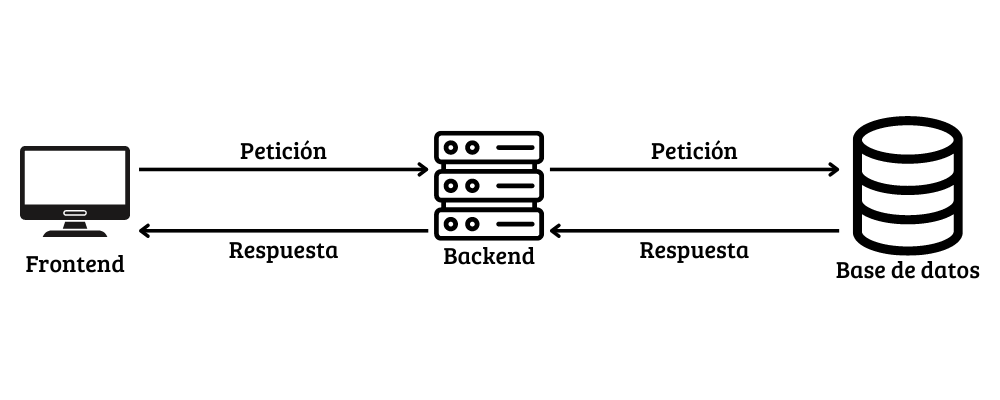
\includegraphics[width=\linewidth]{Imágenes/arquitectura simplificada.png}
\end{document}